%\documentclass[fleqn, 12pt]{article}
\documentclass[fleqn, a4paper, 12pt]{article} %untuk soal

\newcommand\mylog[1]{\mathop{{}^{#1}\mathrm{log}}}

\usepackage[textwidth=330px]{geometry}  %untuk soal
\usepackage{amsmath}
\usepackage{amssymb}
\usepackage{graphicx}
\usepackage{color}
\usepackage{hyperref}
\usepackage{tikz}
\usetikzlibrary{arrows.meta}
\usepackage{pst-plot}
\usepackage{multirow}
\usepackage{verbatim}
\usepackage{longtable}
\usepackage{xcolor}
\usepackage{enumerate}
\usepackage{pgf}
%\usepackage{pgfplots}	%matikan ini untuk soal
\usepackage{multicol}
\usepackage{xfrac}
\hypersetup{
    colorlinks,
    linkcolor={red!50!black},
    citecolor={blue!50!black},
    urlcolor={blue!80!black}
}

\title{Relasi dan Fungsi}
\author{Wisnu OPS}

\begin{document}

\maketitle

\tableofcontents

\section{Relasi}

	Konsep yang dicakup:
	\begin{enumerate}
		\item Pengenalan terhadap konsep relasi dua himpunan
		\item Himpunan penyelesaian dan grafik
		\item Menyatakan relasi sebagai himpunan pasangan terurut
		\item Konsep Domain dan Range
		\item Jenis-jenis relasi; relasi invers, refleksif, simetris, antisimetris, transitif, dan ekuivalensi.
	\end{enumerate}
	
	\newpage
	
	\textbf{Soal-soal Relasi - 1}
	
	\begin{enumerate}
		\item Diketahui relasi berikut ini:	\\
			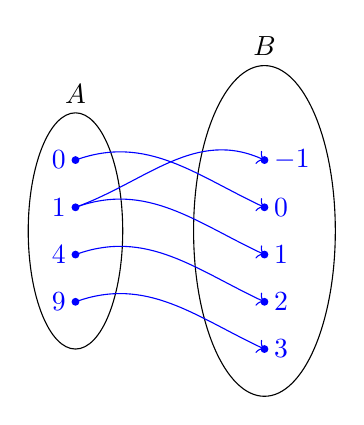
\begin{tikzpicture}[scale=0.6]				
				\draw (1, 2) node[above] {$A$};
				\draw (5, 3) node[above] {$B$};
				\draw (1, -0.5) ellipse (1 and 2.5);
				\draw (5, -0.5) ellipse (1.5 and 3.5);
				\draw[fill, color=blue] (1, 1) circle (2pt) node[left] {$0$};
				\draw[fill, color=blue] (1, 0) circle (2pt) node[left] {$1$};
				\draw[fill, color=blue] (1, -1) circle (2pt) node[left] {$4$};
				\draw[fill, color=blue] (1, -2) circle (2pt) node[left] {$9$};
				\draw[fill, color=blue] (5, 1) circle (2pt) node[right] {$-1$};
				\draw[fill, color=blue] (5, 0) circle (2pt) node[right] {$0$};
				\draw[fill, color=blue] (5, -1) circle (2pt) node[right] {$1$};
				\draw[fill, color=blue] (5, -2) circle (2pt) node[right] {$2$};
				\draw[fill, color=blue] (5, -3) circle (2pt) node[right] {$3$};
				\draw[->, color=blue] (1, 1) to[out=20, in=155] (5, 0);
				\draw[->, color=blue] (1, 0) to[out=20, in=155] (5, 1);
				\draw[->, color=blue] (1, 0) to[out=20, in=155] (5, -1);
				\draw[->, color=blue] (1, -1) to[out=20, in=155] (5, -2);
				\draw[->, color=blue] (1, -2) to[out=20, in=155] (5, -3);
			\end{tikzpicture}
			
			Relasi $R: A \rightarrow B$ \textit{bisa} dinyatakan dalam ....
			
			\begin{enumerate}[(A)]
				\item lebih dari
				\item kurang dari
				\item kuadrat dari
				\item pangkat tiga dari
				\item sama dengan
			\end{enumerate}
			
			\textit{Jawab: C}
		\item Himpunan relasi $R: A \rightarrow B$ yang menunjukkan "faktor prima dari" adalah ...
			\begin{enumerate}[(A)]
				\item $R = \{(1, 6), (2, 6), (3, 6)\}$
				\item $R = \{(2, 6), (3, 12), (7, 7)\}$
				\item $R = \{(2, 6), (3, 12), (1, 7), (7, 7)\}$
				\item $R = \{(2, 6), (3, 6),(2, 12), (3, 12), (1, 7), (7, 7)\}$
				\item $R = \{(2, 6), (3, 6),(2, 12), (3, 12), (7, 7)\}$
			\end{enumerate}
			
			\textit{Jawab: E}
			
		\newpage
			
		\item Diketahui relasi yang dinyatakan diagram berikut:	\\
			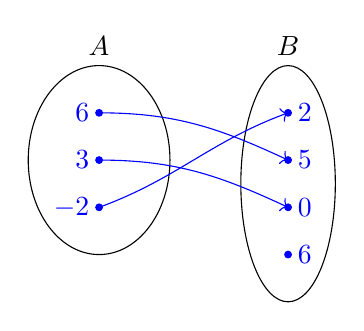
\begin{tikzpicture}[scale=0.6]
				\draw (1, 2) node[above] {$A$};
				\draw (5, 2) node[above] {$B$};
				\draw (1, 0) ellipse (1.5 and 2);
				\draw (5, -0.5) ellipse (1 and 2.5);
				\draw[fill, color=blue] (1, 1) circle (2pt) node[left] {$6$};
				\draw[fill, color=blue] (1, 0) circle (2pt) node[left] {$3$};
				\draw[fill, color=blue] (1, -1) circle (2pt) node[left] {$-2$};
				\draw[fill, color=blue] (5, 1) circle (2pt) node[right] {$2$};
				\draw[fill, color=blue] (5, 0) circle (2pt) node[right] {$5$};
				\draw[fill, color=blue] (5, -1) circle (2pt) node[right] {$0$};
				\draw[fill, color=blue] (5, -2) circle (2pt) node[right] {$6$};
				\draw[->, color=blue] (1, 1) to[out=0, in=155] (5, 0);
				\draw[->, color=blue] (1, 0) to[out=0, in=155] (5, -1);
				\draw[->, color=blue] (1, -1) to[out=20, in=200] (5, 1);
			\end{tikzpicture}

			Range dari relasi tersebut adalah ....
			
			\begin{enumerate}[(A)]
				\item $\{6, 3, -2\}$
				\item $\{2, 5, 0\}$
				\item $\{2, 5, 0, 6\}$
				\item $\{2, 5, 0, 6, 3, -2\}$
				\item $\{2, 5, 0, 6, 6, 3, -2\}$
			\end{enumerate}
			
			\textit{Jawab: B. Sekalian jelasin aja konsep domain di sini. Juga konsep co-domain juga bisa. Cuma harus rada hati-hati. Untuk himpunan A, nggak ada term yang bisa membedakan antara konsep range dan kodomain seperti di himpunan B}
		
		\newpage
		
		\item Diketahui relasi $R:A \rightarrow B$ yang dinyatakan dalam bentuk grafik berikut (setiap kotak menunjukkan satu satuan):	\\
			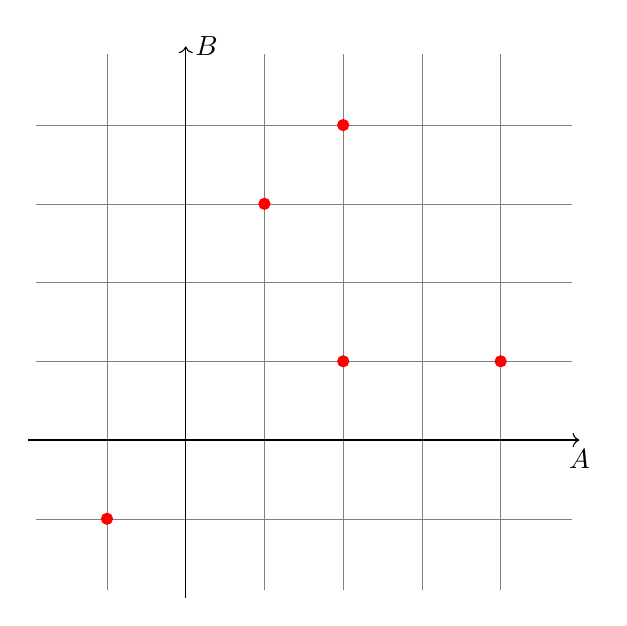
\begin{tikzpicture}
				\draw[color=gray, very thin] (-1.9, -1.9) grid (4.9, 4.9);
				\draw[->] (-2, 0) -- (5, 0) node[below] {$A$};
				\draw[->] (0, -2) -- (0, 5) node[right] {$B$};
				\draw[color=red, fill] (-1, -1) circle (2pt);
				\draw[color=red, fill] (1, 3) circle (2pt);
				\draw[color=red, fill] (2, 1) circle (2pt);
				\draw[color=red, fill] (2, 4) circle (2pt);
				\draw[color=red, fill] (4, 1) circle (2pt);
			\end{tikzpicture}
			
			Range dari relasi tersebut adalah ....
			
			\begin{enumerate}[(A)]
				\item $\{-1, 1, 3, 4\}$
				\item $\{-1, 1, 1, 3, 4\}$
				\item $\{-1, 1, 2, 4\}$
				\item $\{-1, 1, 2, 3, 4\}$
				\item $\{-1, 1, 1, 2, 4\}$
			\end{enumerate}
			
			\textit{Jawab: A}
		
		\newpage
		
		\item Diketahui relasi $R:x \rightarrow y$ yang dinyatakan dalam bentuk grafik berikut (setiap kotak menunjukkan satu satuan):	\\
			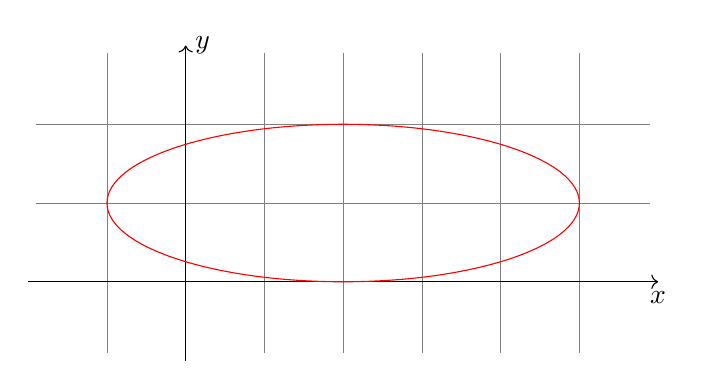
\begin{tikzpicture}
				\draw[color=gray, very thin] (-1.9, -0.9) grid (5.9, 2.9);
				\draw[->] (-2, 0) -- (6, 0) node[below] {$x$};
				\draw[->] (0, -1) -- (0, 3) node[right] {$y$};
				\draw[color=red] (2, 1) ellipse (3 and 1);
			\end{tikzpicture}
			
			Domain dari relasi tersebut adalah ....
			
			\begin{enumerate}[(A)]
				\item $ 0 \leq y \leq 2$
				\item $ -1 \leq y \leq 5$
				\item $ 0 \leq x \leq 2$
				\item $ -1 \leq x \leq 5$
				\item $ 0 \leq x \leq 5$
			\end{enumerate}
			
			\textit{Jawab: D}
			
		\item Diketahui relasi $R:A \rightarrow B$ yang dinyatakan dalam bentuk himpunan penyelesaian $HP = R = \{(1, 2), (2, 3), (4, 5), (6, 5)\}$. Invers dari relasi tersebut adalah?
		
			\begin{enumerate}[(A)]
				\item $R^{-1} = \{(1, 2), (2, 3), (4, 5), (6, 5)\}$
				\item $R^{-1} = \{(2, 1), (2, 3), (4, 5), (6, 5)\}$
				\item $R^{-1} = \{(2, 1), (3, 2), (4, 5), (6, 5)\}$
				\item $R^{-1} = \{(2, 1), (3, 2), (5, 4), (6, 5)\}$
				\item $R^{-1} = \{(2, 1), (3, 2), (5, 4), (5, 6)\}$
				\item $R^{-1} = \{(2, 1), (3, 2), (5, 4)\}$
			\end{enumerate}
		
		\newpage
		
		\item Di antara tiga relasi berikut ini:
		
			\begin{enumerate}[(1)]
				\item $R: x \rightarrow y$ dengan $x \geq y$
				\item $R: x \rightarrow y$ dengan $x > y$
				\item $R: A \rightarrow B$ dengan $A = \{1, 2, 3\}$ dan \\ $R = \{(1, 1), (1, 2), (2, 2), (2, 3), (3, 3), (3, 4)\}$
			\end{enumerate}
			
			Yang manakah yang merupakan relasi yang reflektif?
			
			\begin{enumerate}[(A)]
				\item 1 dan 2 
				\item 1 dan 3
				\item 2 dan 3
				\item 1, 2, dan 3
				\item 3 saja
			\end{enumerate}
			
			\textit{Jawab: B}
		
		\item Diketahui suatu relasi $R: A \rightarrow B$ dinyatakan dalam himpunan penyelesaian $R = \{(1, 4), (2, 3), (3, 2), (4, 1), (2, 6)\}$. Agar relasi tersebut menjadi relasi yang simetris, maka anggota himpunan penyelesaiannya perlu ditambah lagi dengan ....
		
			\begin{enumerate}[(A)]	
				\item $(1, 2)$
				\item $(2, 4)$
				\item $(2, 5)$
				\item $(5, 2)$
				\item $(6, 2)$
			\end{enumerate}
			
			\textit{Jawab: E}
			
		\newpage
		
		\item Di antara tiga relasi berikut ini:
		
			\begin{enumerate}[(1)]
				\item $R: x \rightarrow y$ dengan $x \geq y$
				\item $R: x \rightarrow y$ dengan $x > y$
				\item Relasi antara $x$ dan $y$ yang tergambarkan dengan lingkaran dengan pusat di $(2,2)$ dan jari-jari 1.
			\end{enumerate}
			
			Yang manakah yang merupakan relasi yang antisimetris?
			
			\begin{enumerate}[(A)]
				\item 1 dan 2 
				\item 1 dan 3
				\item 2 dan 3
				\item 1, 2, dan 3
				\item 3 saja
			\end{enumerate}
			
			\textit{Jawab: A. Note: mereka masih kelas 1 dan belum belajar persamaan lingkaran. Jadi nanti ngebahasnya jangan pakai persamaan lingkaran, pakai gambar aja.}
		
		\item Pada relasi $R: x \rightarrow y$ dengan relasi "kurang dari" selalu dipenuhi hal berikut: untuk setiap $(a, b) \in R$ dan $(b, c) \in R$, berlaku juga $(a, c) \in R$. Contoh, jika $a < b$ dan $b < c$, maka berlaku juga $a < c$. Relasi ini adalah relasi ....
		
			\begin{enumerate}[(A)]
				\item Invers
				\item Reflektif
				\item Simetris
				\item Transitif
				\item Ekuivalensi
			\end{enumerate}
			
			\textit{Jawab: D. Btw, materi terakhir yang belum ada soalnya itu relasi ekuivalensi. Jadi di pembahasan ini sekalian kasih tau aja secara singkat tentang relasi ekuivalensi. Relasi ekuivalensi itu adalah relasi yang reflektif, simetris, dan transitif. Contohnya relasi "X sebangun dengan Y" (untuk X dan Y himpunan segitiga)}
	\end{enumerate}
	
\section{Fungsi}

	\subsection{Fungsi}
	
	Konsep yang dicakup:
	
	\begin{enumerate}
		\item Definisi Fungsi; Relasi $R: A \rightarrow B$ disebut fungsi jika setiap anggota dari himpunan $A$ dapat dipasangkan dengan tepat satu unsur di himpunan $B$.
		\item Menyatakan suatu fungsi. Misalkan, luas dinyatakan dalam suatu fungsi panjang. Fungsi-fungsi ini bisa dinyatakan dalam bentuk: diagram anak panah, himpunan pasangan terurut, dan pada koordinat kartesius.		
	\end{enumerate}
	
	\newpage
	
	\textbf{Soal-soal Fungsi - 1}
	
	\begin{enumerate}
		\item Di antara ketiga diagram panah berikut ini, manakah yang merupakan fungsi?
			\begin{enumerate}[I.]
				\item . \\
					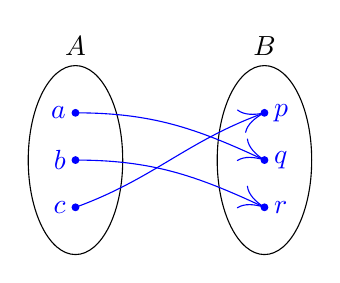
\begin{tikzpicture}[scale=0.6]
						\draw (1, 2) node[above] {$A$};
						\draw (5, 2) node[above] {$B$};
						\draw (1, 0) ellipse (1 and 2);
						\draw (5, 0) ellipse (1 and 2);
						\draw[fill, color=blue] (1, 1) circle (2pt) node[left] {$a$};
						\draw[fill, color=blue] (1, 0) circle (2pt) node[left] {$b$};
						\draw[fill, color=blue] (1, -1) circle (2pt) node[left] {$c$};
						\draw[fill, color=blue] (5, 1) circle (2pt) node[right] {$p$};
						\draw[fill, color=blue] (5, 0) circle (2pt) node[right] {$q$};
						\draw[fill, color=blue] (5, -1) circle (2pt) node[right] {$r$};
						\draw[-{>[scale=3,length=3,width=3]}, color=blue] (1, 1) to[out=0, in=155] (5, 0);
						\draw[-{>[scale=3,length=3,width=3]}, color=blue] (1, 0) to[out=0, in=155] (5, -1);
						\draw[-{>[scale=3,length=3,width=3]}, color=blue] (1, -1) to[out=20, in=200] (5, 1);
					\end{tikzpicture}
				\item . \\
					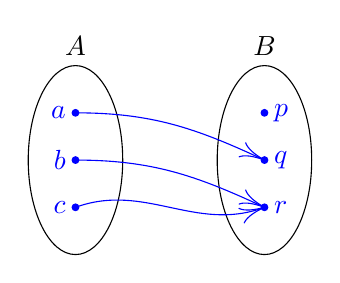
\begin{tikzpicture}[scale=0.6]
						\draw (1, 2) node[above] {$A$};
						\draw (5, 2) node[above] {$B$};
						\draw (1, 0) ellipse (1 and 2);
						\draw (5, 0) ellipse (1 and 2);
						\draw[fill, color=blue] (1, 1) circle (2pt) node[left] {$a$};
						\draw[fill, color=blue] (1, 0) circle (2pt) node[left] {$b$};
						\draw[fill, color=blue] (1, -1) circle (2pt) node[left] {$c$};
						\draw[fill, color=blue] (5, 1) circle (2pt) node[right] {$p$};
						\draw[fill, color=blue] (5, 0) circle (2pt) node[right] {$q$};
						\draw[fill, color=blue] (5, -1) circle (2pt) node[right] {$r$};
						\draw[-{>[scale=3,length=3,width=2]}, color=blue] (1, 1) to[out=0, in=155] (5, 0);
						\draw[-{>[scale=3,length=3,width=2]}, color=blue] (1, 0) to[out=0, in=155] (5, -1);
						\draw[-{>[scale=3,length=3,width=2]}, color=blue] (1, -1) to[out=20, in=200] (5, -1);
					\end{tikzpicture}
				\item . \\
					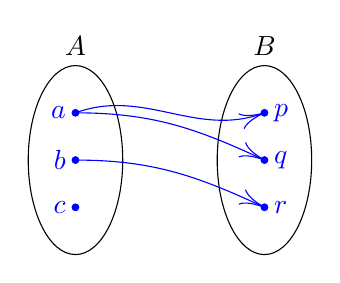
\begin{tikzpicture}[scale=0.6]
						\draw (1, 2) node[above] {$A$};
						\draw (5, 2) node[above] {$B$};
						\draw (1, 0) ellipse (1 and 2);
						\draw (5, 0) ellipse (1 and 2);
						\draw[fill, color=blue] (1, 1) circle (2pt) node[left] {$a$};
						\draw[fill, color=blue] (1, 0) circle (2pt) node[left] {$b$};
						\draw[fill, color=blue] (1, -1) circle (2pt) node[left] {$c$};
						\draw[fill, color=blue] (5, 1) circle (2pt) node[right] {$p$};
						\draw[fill, color=blue] (5, 0) circle (2pt) node[right] {$q$};
						\draw[fill, color=blue] (5, -1) circle (2pt) node[right] {$r$};
						\draw[-{>[scale=3,length=3,width=2]}, color=blue] (1, 1) to[out=0, in=155] (5, 0);
						\draw[-{>[scale=3,length=3,width=2]}, color=blue] (1, 0) to[out=0, in=155] (5, -1);
						\draw[-{>[scale=3,length=3,width=2]}, color=blue] (1, 1) to[out=20, in=200] (5, 1);
					\end{tikzpicture}
				\begin{enumerate}[(A)]
					\item Diagram I saja
					\item Diagram II saja
					\item Diagram III saja
					\item Diagram I dan II saja
					\item Diagram I, II, dan III
				\end{enumerate}
			\end{enumerate}
		
		\newpage
		
		\item Di antara himpunan pasangan terurut di bawah ini, manakah yang merupakan fungsi?
			\begin{enumerate}[(A)]
				\item $A = \{(1, 2), (3, 4), (5, 6), (5, 4), (3, 2)\}$
				\item $B = \{(a, b), (c, d), (e, f), (g, f), (e, d)\}$
				\item $C = \{(1, 3), (5, 7), (9, 8), (9, 4), (2, 1)\}$
				\item $D = \{(-1, 1), (0, 0), (1, 1), (2, 4), (3, 9)\}$
				\item $E = \{(-2, 4), (-1, 1), (0, 0), (1, 1), (1, 2)\}$
			\end{enumerate}
		\item Di antara relasi $x$ dan $y$ berikut ini, manakah yang bisa dinyatakan dalam $y$ sebagai fungsi dari $x$ ($y = f(x)$)?
			\begin{enumerate}[(A)]
				\item $2x + y^2 = 0$
				\item $x^2 + y^2 = 25$
				\item $x^2 - y = 0$
				\item $x^4 + y^4 = 32$
				\item $y^2 = 16x$
			\end{enumerate}
		
		\newpage
		
		\item Di antara grafik pada koordinat kartesius di bawah ini, manakah yang merupakan fungsi $y = f(x)$?
			\begin{enumerate}[I.]
				\item . \\
					\begin{tikzpicture}[scale=0.4]						
						\draw[->] (-1, 0) -- (8, 0) node[below] {$x$};
						\draw[->] (0, -1) -- (0, 5) node[left] {$y$};
						\draw[color=blue] (-1, 4) -- (7, -1);
					\end{tikzpicture}
				\item . \\
					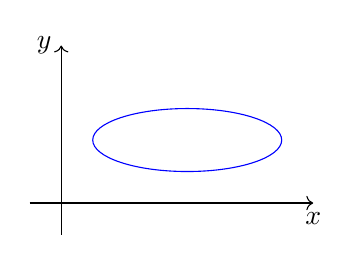
\begin{tikzpicture}[scale=0.4]						
						\draw[->] (-1, 0) -- (8, 0) node[below] {$x$};
						\draw[->] (0, -1) -- (0, 5) node[left] {$y$};
						\draw[color=blue] (4, 2) ellipse (3 and 1);
					\end{tikzpicture}
				\item . \\
					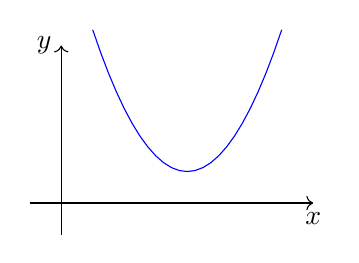
\begin{tikzpicture}[scale=0.4]
						\draw[->] (-1, 0) -- (8, 0) node[below] {$x$};
						\draw[->] (0, -1) -- (0, 5) node[left] {$y$};
						\draw[domain=1:7, variable=\x, color=blue] plot({\x}, {(\x-4)*(\x-4)/2 + 1});
					\end{tikzpicture}
				\item . \\
					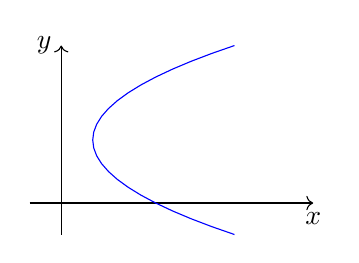
\begin{tikzpicture}[scale=0.4]						
						\draw[->] (-1, 0) -- (8, 0) node[below] {$x$};
						\draw[->] (0, -1) -- (0, 5) node[left] {$y$};
						\draw[domain=-1:5, variable=\y, color=blue] plot({(\y-2)*(\y-2)/2 + 1}, {\y});
					\end{tikzpicture}
			\end{enumerate}
			\begin{enumerate}[(A)]
				\item I, II, dan III
				\item I dan III
				\item II dan IV
				\item IV saja
				\item I, II, III, dan IV
			\end{enumerate}
		
		\newpage
		
		\item Diketahui $f(x) = 3x^2 + 4$, $g(x) = 7$, dan $h = \{(2, 5), (3, 5), (4, 5)\}$. Pernyataan berikut ini yang benar adalah ....
		\begin{enumerate}[(A)]
			\item Hanya $f$ yang merupakan fungsi
			\item Hanya $g$ yang merupakan fungsi
			\item Hanya $h$ yang merupakan fungsi
			\item Hanya $f$ dan $g$ yang merupakan fungsi
			\item $f$, $g$, dan $h$ adalah fungsi
		\end{enumerate}
		\item Diketahui $A = \{(3, 4), (5, 6), (4, 7), (1, 2), (3, 9)\}$. Agar $A$ menjadi sebuah fungsi, pasangan yang harus dibalik kedudukannya ($(a, b)$ dibalik menjadi $(b, a)$) adalah ....
		\begin{enumerate}[(A)]
			\item $(3, 4)$
			\item $(5, 6)$
			\item $(4, 7)$
			\item $(1, 2)$
			\item $(3, 9)$
		\end{enumerate}
		\item Suatu balok memiliki panjang $x$, lebar setengah kali panjangnya, dan tinggi 20 satuan. Volume balok dapat dinyatakan sebagai fungsi dari $x$ sebagai berikut:
			\begin{enumerate}[(A)]
				\item $V(x) = 10x^2$
				\item $V(x) = x (x - 20)$
				\item $V(x) = \frac{x (x - 20)}{2}$
				\item $V(x) = 10x$
				\item $V(x) = 5x^3$
			\end{enumerate}
	\end{enumerate}
	
	\subsection{Produk Himpunan dan Jenis-jenis Fungsi}
	
	\begin{enumerate}
		\item Produk himpunan $A \times B$		
		\item Jenis-jenis fungsi
			\begin{enumerate}[a.]
				\item Fungsi Surjective; Nama lainnya itu fungsi Onto
				\item Fungsi Injective; Nama lainnya itu fungsi satu-satu atau fungsi one-to-one
				\item Fungsi Bijective; Fungsi Bijective itu adalah fungsi yang surjective dan juga injective. Nama lainnya itu fungsi korespondensi satu-satu atau one-to-one correspondence.
				\item \textbf{Catatan Penting: Bedain antara fungsi satu-satu sama fungsi korespondensi satu-satu}. Buku Sukino salah karena dua hal itu dianggap sama. Mungkin perlu dikasih tau kalau bisa aja yang gurunya ajarin itu salah kalau mereka pakai buku yang salah.
			\end{enumerate}
		\item Suatu fungsi itu pasti memiliki invers kalau dia merupakan fungsi injective.
	\end{enumerate}
	
	\textbf{Soal-soal Fungsi - 2}
	
	\begin{enumerate}
		\item Jika $n(A) = 2$ dan $n(B) = 5$, maka $n(A \times B) = $ ....
		\begin{enumerate}[(A)]
			\item 2
			\item 7
			\item 10
			\item 25
			\item 32
		\end{enumerate}
		\item Diketahui $A = \{5, 6\}$ dan $B = \{1, 3, 7\}$. Banyaknya anggota dari $A \times B$ adalah ....
		\begin{enumerate}[(A)]
			\item 2 buah
			\item 3 buah
			\item 4 buah
			\item 6 buah
			\item 8 buah
		\end{enumerate}
		\item Jika $x < 0$ dan $x \cdot y > 0$, titik $(x, y)$ terletak di kuadran ....
		\begin{enumerate}[(A)]
			\item I
			\item II
			\item III
			\item IV
			\item I dan II
		\end{enumerate}
		
		\newpage
		
		\item Jika $y > 0$ dan $x \cdot y < 0$, titik $(x, y)$ terletak di kuadran ....
		\begin{enumerate}[(A)]
			\item I
			\item II
			\item III
			\item IV
			\item III dan IV
		\end{enumerate}
		
		\item Diagram berikut ini yang menunjukkan fungsi apa?	\\
			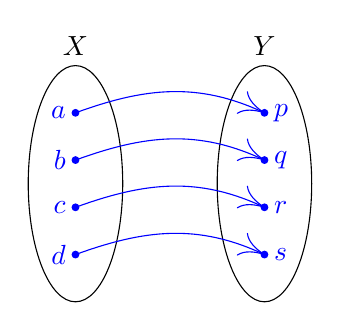
\begin{tikzpicture}[scale=0.6]
				\draw (1, 2) node[above] {$X$};
				\draw (5, 2) node[above] {$Y$};
				\draw (1, -0.5) ellipse (1 and 2.5);
				\draw (5, -0.5) ellipse (1 and 2.5);
				\draw[fill, color=blue] (1, 1) circle (2pt) node[left] {$a$};
				\draw[fill, color=blue] (1, 0) circle (2pt) node[left] {$b$};
				\draw[fill, color=blue] (1, -1) circle (2pt) node[left] {$c$};
				\draw[fill, color=blue] (1, -2) circle (2pt) node[left] {$d$};
				\draw[fill, color=blue] (5, 1) circle (2pt) node[right] {$p$};
				\draw[fill, color=blue] (5, 0) circle (2pt) node[right] {$q$};
				\draw[fill, color=blue] (5, -1) circle (2pt) node[right] {$r$};
				\draw[fill, color=blue] (5, -2) circle (2pt) node[right] {$s$};
				\draw[-{>[scale=3,length=3,width=3]}, color=blue] (1, 1) to[out=20, in=155] (5, 1);
				\draw[-{>[scale=3,length=3,width=3]}, color=blue] (1, 0) to[out=20, in=155] (5, 0);
				\draw[-{>[scale=3,length=3,width=3]}, color=blue] (1, -1) to[out=20, in=155] (5, -1);
				\draw[-{>[scale=3,length=3,width=3]}, color=blue] (1, -2) to[out=20, in=155] (5, -2);
			\end{tikzpicture}
			\begin{enumerate}[(A)]
				\item Fungsi surjective (onto) dan injective (one-to-one)
				\item Fungsi surjective dan non-injective
				\item Fungsi non-surjective dan injecitve
				\item Fungsi non-surjective dan non-injective
				\item Bukan Fungsi
			\end{enumerate}
		\item Diagram berikut ini yang menunjukkan fungsi apa?	\\
			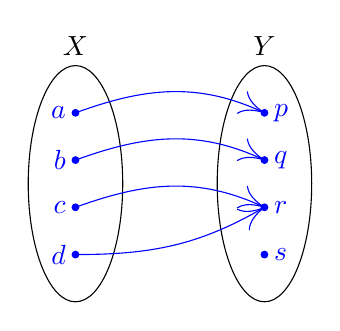
\begin{tikzpicture}[scale=0.6]
				\draw (1, 2) node[above] {$X$};
				\draw (5, 2) node[above] {$Y$};
				\draw (1, -0.5) ellipse (1 and 2.5);
				\draw (5, -0.5) ellipse (1 and 2.5);
				\draw[fill, color=blue] (1, 1) circle (2pt) node[left] {$a$};
				\draw[fill, color=blue] (1, 0) circle (2pt) node[left] {$b$};
				\draw[fill, color=blue] (1, -1) circle (2pt) node[left] {$c$};
				\draw[fill, color=blue] (1, -2) circle (2pt) node[left] {$d$};
				\draw[fill, color=blue] (5, 1) circle (2pt) node[right] {$p$};
				\draw[fill, color=blue] (5, 0) circle (2pt) node[right] {$q$};
				\draw[fill, color=blue] (5, -1) circle (2pt) node[right] {$r$};
				\draw[fill, color=blue] (5, -2) circle (2pt) node[right] {$s$};
				\draw[-{>[scale=3,length=3,width=3]}, color=blue] (1, 1) to[out=20, in=155] (5, 1);
				\draw[-{>[scale=3,length=3,width=3]}, color=blue] (1, 0) to[out=20, in=155] (5, 0);
				\draw[-{>[scale=3,length=3,width=3]}, color=blue] (1, -1) to[out=20, in=155] (5, -1);
				\draw[-{>[scale=3,length=3,width=3]}, color=blue] (1, -2) to[out=0, in=210] (5, -1);
			\end{tikzpicture}
			\begin{enumerate}[(A)]
				\item Fungsi surjective (onto) dan injective (one-to-one)
				\item Fungsi surjective dan non-injective
				\item Fungsi non-surjective dan injecitve
				\item Fungsi non-surjective dan non-injective
				\item Bukan Fungsi
			\end{enumerate}
		
		\newpage
		
		\item Diagram berikut ini yang menunjukkan fungsi apa?	\\
			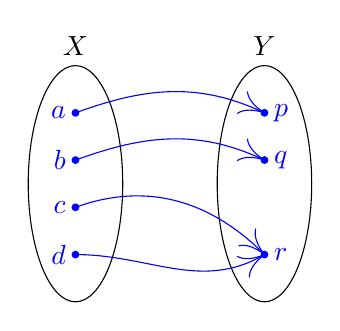
\begin{tikzpicture}[scale=0.6]
				\draw (1, 2) node[above] {$X$};
				\draw (5, 2) node[above] {$Y$};
				\draw (1, -0.5) ellipse (1 and 2.5);
				\draw (5, -0.5) ellipse (1 and 2.5);
				\draw[fill, color=blue] (1, 1) circle (2pt) node[left] {$a$};
				\draw[fill, color=blue] (1, 0) circle (2pt) node[left] {$b$};
				\draw[fill, color=blue] (1, -1) circle (2pt) node[left] {$c$};
				\draw[fill, color=blue] (1, -2) circle (2pt) node[left] {$d$};
				\draw[fill, color=blue] (5, 1) circle (2pt) node[right] {$p$};
				\draw[fill, color=blue] (5, 0) circle (2pt) node[right] {$q$};				
				\draw[fill, color=blue] (5, -2) circle (2pt) node[right] {$r$};
				\draw[-{>[scale=3,length=3,width=3]}, color=blue] (1, 1) to[out=20, in=155] (5, 1);
				\draw[-{>[scale=3,length=3,width=3]}, color=blue] (1, 0) to[out=20, in=155] (5, 0);
				\draw[-{>[scale=3,length=3,width=3]}, color=blue] (1, -1) to[out=20, in=135] (5, -2);
				\draw[-{>[scale=3,length=3,width=3]}, color=blue] (1, -2) to[out=0, in=210] (5, -2);
			\end{tikzpicture}
			\begin{enumerate}[(A)]
				\item Fungsi surjective (onto) dan injective (one-to-one)
				\item Fungsi surjective dan non-injective
				\item Fungsi non-surjective dan injecitve
				\item Fungsi non-surjective dan non-injective
				\item Bukan Fungsi
			\end{enumerate}
		\item Diagram berikut ini yang menunjukkan fungsi apa?	\\
			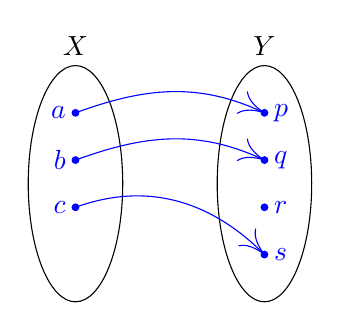
\begin{tikzpicture}[scale=0.6]
				\draw (1, 2) node[above] {$X$};
				\draw (5, 2) node[above] {$Y$};
				\draw (1, -0.5) ellipse (1 and 2.5);
				\draw (5, -0.5) ellipse (1 and 2.5);
				\draw[fill, color=blue] (1, 1) circle (2pt) node[left] {$a$};
				\draw[fill, color=blue] (1, 0) circle (2pt) node[left] {$b$};
				\draw[fill, color=blue] (1, -1) circle (2pt) node[left] {$c$};				
				\draw[fill, color=blue] (5, 1) circle (2pt) node[right] {$p$};
				\draw[fill, color=blue] (5, 0) circle (2pt) node[right] {$q$};				
				\draw[fill, color=blue] (5, -1) circle (2pt) node[right] {$r$};
				\draw[fill, color=blue] (5, -2) circle (2pt) node[right] {$s$};
				\draw[-{>[scale=3,length=3,width=3]}, color=blue] (1, 1) to[out=20, in=155] (5, 1);
				\draw[-{>[scale=3,length=3,width=3]}, color=blue] (1, 0) to[out=20, in=155] (5, 0);
				\draw[-{>[scale=3,length=3,width=3]}, color=blue] (1, -1) to[out=20, in=135] (5, -2);				
			\end{tikzpicture}
			\begin{enumerate}[(A)]
				\item Fungsi surjective (onto) dan injective (one-to-one)
				\item Fungsi surjective dan non-injective
				\item Fungsi non-surjective dan injecitve
				\item Fungsi non-surjective dan non-injective
				\item Bukan Fungsi
			\end{enumerate}		
		
		\newpage
		
		\item Fungsi $f: R \rightarrow R$, dengan $R$ himpunan bilangan real. Berikut yang merupakan fungsi injective yang non-surjective adalah ....
		\begin{enumerate}[(A)]
			\item $f(x) = x^4$
			\item $f(x) = x^2$
			\item $f(x) = |x|$
			\item $f(x) = \frac{1}{2}x + 6$
			\item $f(x) = 2^x$
		\end{enumerate}
		
		\textit{Jawabannya yang E. Kalau yang D itu injective dan surjective}
		
		\item Jika $n(P) = n(Q) = 5$, maka $n(f: P \xrightarrow{bijective} Q) = $ ....
		\begin{enumerate}[(A)]
			\item 5
			\item 25
			\item 75
			\item 100
			\item 120
		\end{enumerate}
		
		\item Jika $n(f: A \xrightarrow{bijective} A) = 24$, maka $n(A) = $ ....
		\begin{enumerate}[(A)]
			\item 1
			\item 2
			\item 3
			\item 4
			\item 5
		\end{enumerate}
		
		\item Di antara himpunan pasangan terurut di bawah ini, manakah yang merupakan fungsi yang memiliki invers?
			\begin{enumerate}[(A)]
				\item $A = \{(1, 2), (3, 4), (5, 6), (6, 4), (7, 2)\}$
				\item $B = \{(a, b), (c, d), (e, f), (g, f), (h, d)\}$
				\item $C = \{(1, 3), (5, 7), (9, 8), (9, 4), (2, 1)\}$
				\item $D = \{(-1, -1), (0, 0), (1, 1), (2, 4), (3, 9)\}$
				\item $E = \{(-2, 4), (-1, 1), (0, 0), (1, 1), (1, 2)\}$
			\end{enumerate}
		
		\newpage
		
		\item Suatu fungsi pasti memiliki invers jika dan hanya jika ....
		\begin{enumerate}[(A)]
			\item Fungsi tersebut fungsi surjective 
			\item Fungsi tersebut fungsi injective 
			\item Fungsi tersebut fungsi surjective and injective (bijective)
			\item Semua fungsi memiliki invers
			\item A, B, C, dan D salah
		\end{enumerate}
		
		\item Jika $A = \{1, 3, 5, 7\}$ dan $B = \{2, 3, 5\}$, maka $n(f: A \rightarrow B) = $ ....
		\begin{enumerate}[(A)]
			\item 7
			\item 12
			\item 64
			\item 81
			\item 115
		\end{enumerate}
		\item Jika $A = \{1, 3, 5, 7\}$ dan $B = \{2, 3, 5\}$, maka $n(f: B \rightarrow A) = $ ....
		\begin{enumerate}[(A)]
			\item 7
			\item 12
			\item 64
			\item 81
			\item 115
		\end{enumerate}		
		
		\newpage
		
		\item Diketahui $S = \{2, 4, 6, 8\}$ dan $T = \{2, 3, 5\}$. Jika $f = \{(2, 2), (4, 5), (8, 3)\}$, maka $f$ adalah ....
		\begin{enumerate}[(A)]
			\item fungsi, tapi bukan surjective maupun injective
			\item fungsi injective
			\item fungsi surjective
			\item relasi, tapi bukan relasi ekuivalensi
			\item relasi ekuivalensi
		\end{enumerate}
	\end{enumerate}
	
	\subsection{Menghitung Nilai Fungsi, Domain, dan Range}
	
		Konsep subbab ini:
		
		\begin{enumerate}
			\item Domain, Kodomain, dan Range
			\item Menghitung Nilai Fungsi satu variabel
			\item Menghitung Nilai Fungsi multivariabel
			\item Fungsi ganjil dan Fungsi genap			
		\end{enumerate}
	
	\textbf{Soal-soal 3}
	
	\begin{enumerate}
		\item Suatu fungsi $f: A \rightarrow B$ dengan $A = \{-3, -2, -1, 0, 1, 2, 3\}$ dan $B = \{0, 1, 2, 3, 4, 5, 6, 7, 8, 9\}$, terdefinisi $f(x) = x^2$. Tentukan range fungsi tersebut!
			\begin{enumerate}[(A)]
				\item $\{0, 1, 4, 6, 9\}$
				\item $\{-3, -2, -1, 0, 1, 2, 3, 4, 5, 6, 7, 8, 9\}$
				\item $\{0, 1, 2, 3, 4, 5, 6, 7, 8, 9\}$
				\item $\{0, 1, 4, 9\}$
				\item $\{1, 2, 3, 4, 5, 6, 7, 8, 9\}$
			\end{enumerate}
		
		\newpage
		
		\item Suatu fungsi $f: A \rightarrow B$ dengan $A = \{-3, -2, -1, 0, 1, 2, 3\}$ dan $B = \{0, 1, 2, 3, 4, 5, 6, 7, 8, 9\}$, terdefinisi $f(x) = x^2$. Tentukan range fungsi tersebut!
			\begin{enumerate}[(A)]
				\item $\{0, 1, 4, 6, 9\}$
				\item $\{-3, -2, -1, 0, 1, 2, 3, 4, 5, 6, 7, 8, 9\}$
				\item $\{0, 1, 2, 3, 4, 5, 6, 7, 8, 9\}$
				\item $\{0, 1, 4, 9\}$
				\item $\{1, 2, 3, 4, 5, 6, 7, 8, 9\}$
			\end{enumerate}
		\item Suatu fungsi $f: R \rightarrow R$ dengan $R$ adalah himpunan anggota bilangan real dan terdefinisi $f(x) = x^2 - 4x + 3$. Tentukan range dari fungsi tersebut!
			\begin{enumerate}[(A)]
				\item $\{y | y \geq -1, y \in \mathbb{R}\}$
				\item $\{y | y \leq -1, y \in \mathbb{R}\}$
				\item $\{y | y \geq 1, y \in \mathbb{R}\}$
				\item $\{y | y \leq 1, y \in \mathbb{R}\}$
				\item $\{y | -1 \leq y \leq 1, y \in \mathbb{R}\}$
			\end{enumerate}
		\item Suatu fungsi $f(x) = x^2 - 6x + 5$ memiliki domain $D = \{x | 5 \leq x \leq 7, x \in \mathbb{R}\}$. Tentukan range dari fungsi tersebut!
			\begin{enumerate}[(A)]
				\item $\{y | -4 \leq y \leq 12, y \in \mathbb{R}\}$
				\item $\{y | 0 \leq y \leq 12, y \in \mathbb{R}\}$
				\item $\{y | -4 \leq y \leq 0, y \in \mathbb{R}\}$
				\item $\{y | 4 \leq y \leq 7, y \in \mathbb{R}\}$
				\item $\{y | 5 \leq y \leq 7, y \in \mathbb{R}\}$
			\end{enumerate}
		\item Suatu fungsi $f(x) = x^2 - 6x + 5$ memiliki domain $D = \{x | 0 \leq x \leq 1, x \in \mathbb{R}\}$. Tentukan range dari fungsi tersebut!
			\begin{enumerate}[(A)]
				\item $\{y | 5 \leq y \leq 0, y \in \mathbb{R}\}$
				\item $\{y | 0 \leq y \leq 4, y \in \mathbb{R}\}$
				\item $\{y | 4 \leq y \leq 0, y \in \mathbb{R}\}$
				\item $\{y | 4 \leq y \leq 7, y \in \mathbb{R}\}$
				\item $\{y | 0 \leq y \leq 5, y \in \mathbb{R}\}$
			\end{enumerate}
		
		\newpage
		
		\item Suatu fungsi $f(x) = x^2 - 6x + 5$ memiliki domain $D = \{x | 0 \leq x \leq 7, x \in \mathbb{R}\}$. Tentukan range dari fungsi tersebut!
			\begin{enumerate}[(A)]
				\item $\{y | -4 \leq y \leq 12, y \in \mathbb{R}\}$
				\item $\{y | 0 \leq y \leq 12, y \in \mathbb{R}\}$
				\item $\{y | -4 \leq y \leq 0, y \in \mathbb{R}\}$
				\item $\{y | 4 \leq y \leq 7, y \in \mathbb{R}\}$
				\item $\{y | 5 \leq y \leq 7, y \in \mathbb{R}\}$
			\end{enumerate}
		\item Jika $f(x) = x^3 - x^2 - x - 1$, nilai dari $f(x) = $ ....
			\begin{enumerate}[(A)]
				\item 0
				\item -1
				\item -2
				\item -3
				\item -4
			\end{enumerate}
		\item Jika $f(x) = x^7 - 97x^6 - 199x^5 + 99x^4 - 2x + 190$, nilai $f(99) = $ ....
			\begin{enumerate}[(A)]
				\item -8
				\item -2
				\item 4
				\item 10
				\item 16
			\end{enumerate}
		\item Diketahui $f(x, y, z) = (x + y)(y + z)$. Berapa nilai dari $f(1, -2, 3) = $ ....
			\begin{enumerate}[(A)]
				\item 1
				\item 0
				\item -1
				\item -3
				\item -7
			\end{enumerate}
		
		\newpage
		
		\item Fungsi mutlak $f(x) = |x|$ dapat didefinisikan sebagai berikut:
			\[f(x) = |x| =  \left\{ 
				\begin{array}{l l}
					x & \quad \text{jika $x \geq 0$}\\
					-x & \quad \text{jika $x < 0$}
				\end{array} \right.\]
			Berapakah nilai dari $|a - 10|$ jika $a = 3$?
			\begin{enumerate}[(A)]
				\item -10
				\item -7
				\item -3
				\item 3
				\item 7
			\end{enumerate}
		\item Fungsi genap adalah fungsi yang memenuhi hubungan $f(-x) = f(x)$. Dengan demikian, dari fungsi berikut ini, yang termasuk fungsi genap adalah ....
			\begin{enumerate}[(1)]				
				\item $f(x) = \frac{1}{x^2}$
				\item $f(x) = \frac{1}{x}$
				\item $f(x) = |x|$
				\item $f(x) = \sin x$
			\end{enumerate}
			\begin{enumerate}[(A)]
				\item (1), (2), dan (3)
				\item (1) dan (3)
				\item (2) dan (4)
				\item (4)
				\item (1), (2), (3), dan (4)
			\end{enumerate}
		
		\newpage
		
		\item Fungsi ganjil adalah fungsi yang memenuhi hubungan $f(-x) = -f(x)$. Dengan demikian, dari fungsi berikut ini, yang termasuk fungsi ganjil adalah ....
			\begin{enumerate}[(1)]			
				\item $f(x) = \frac{1}{x}$
				\item $f(x) = \sin x$
				\item $f(x) = x^3$
				\item $f(x) = \cos x$
			\end{enumerate}
			\begin{enumerate}[(A)]
				\item (1), (2), dan (3)
				\item (1) dan (3)
				\item (2) dan (4)
				\item (4)
				\item (1), (2), (3), dan (4)
			\end{enumerate}			
	\end{enumerate}

\end{document}